\subsubsection{Model}
\vspace{-0.5cm}
\begin{figure}[H]
\centering
\includegraphics[width = 1.0  \textwidth]{Figurer/classesModel.pdf}
\caption{Klassediagram over de klasser der bliver brugt i Model-delen af MVC designmønstret.}
\label{fig:classesModel}
\end{figure}

%% MIKKEL %%
% BRÆT????
\textbf{Brættet:} I forhold til \textsc{SimpDam} er der tilføjet følgende booleans til felter af typen \texttt{Tile}: \texttt{highlighted}, \texttt{canBeUsedInCombo} og \texttt{isUsedInCombo}. I stedet for brug af et boolean \texttt{occupied}som i \textsc{SimpDam}, har hvert felt nu direkte forbundet med sin tilhørende brikken. Brættet lagres stadig i \texttt{Tile[][] board}. \\

%% MIKKEL %%
% Hvordan lagres brikker og tiles internt?
\textbf{Brikker:} \texttt{Piece} i \textsc{AvaDam} er en udbygning af \texttt{Piece} i \textsc{SimpDam}: Der er tilføjet følgende booleans:  \texttt{crowned}, \texttt{canKill}, \texttt{canBeKilledInCombo}, \texttt{beingKilledInCombo}. Udover disse har \texttt{Piece} også to farver \texttt{crownedColor} og \texttt{killColor}, der bruges til at sætte kantfarver, samt et felt \texttt{Player}. Vi har tilføjet en \texttt{player} \texttt{None}, svarende til at ingen må flytte brikker (fx når spillet er ovre.) Konstruktøren for brikken tager nu også imod om brikken er kronet. Brikker lagres stadig i ArrayListen \texttt{<Piece> pieces}, og fjernes som i \textsc{SimpDam}. \\

%% MIKKEL %%
% Hvordan lagres spilreglerne?
\textbf{Valgfri regler:} De valgfri regler kan ændres i Settings menuen. Klassen \texttt{ModelSettings} indeholder booleans svarende til disse regler, som set i \ref{fig:settingsMenu}. Når en \texttt{CheckBox} i settings menuen bliver trykket på, opdateres den tilsvarende boolean i \texttt{ModelSettings}. Nogle check boxes sætter flere værdier, såsom \texttt{mustCompleteCombo} der også sætter \texttt{mandatoryFirstKill} til sand (og gør dennes \texttt{CheckBox} inaktiv), da et drab er en combo med længden 1. \\

Når brugeren klikker \texttt{"Start game"}, bruges indstillingerne fra \texttt{ModelSettings} til konstruktørerne af bræt og brikker. Dette udføres af metoden \texttt{loadSettings}. 

Når sliderens værdi ændres i menuen med indstillinger, opdateres den tilknyttede label ved brug af følgende kode:
\begin{lstlisting}
slider.valueProperty().addListener((obs, oldVal, newVal) -> {
    sliderValueLabel.setText("" + (int) slider.getValue());
});
\end{lstlisting}

Dens værdi bliver overført til \texttt{tileAmount} når metoden \texttt{setup} bliver kørt i \texttt{DamModel}, hvor den bliver overført til \texttt{tileAmount} gennem \texttt{slider.getValue}. 

\begin{figure}[H]
\centering
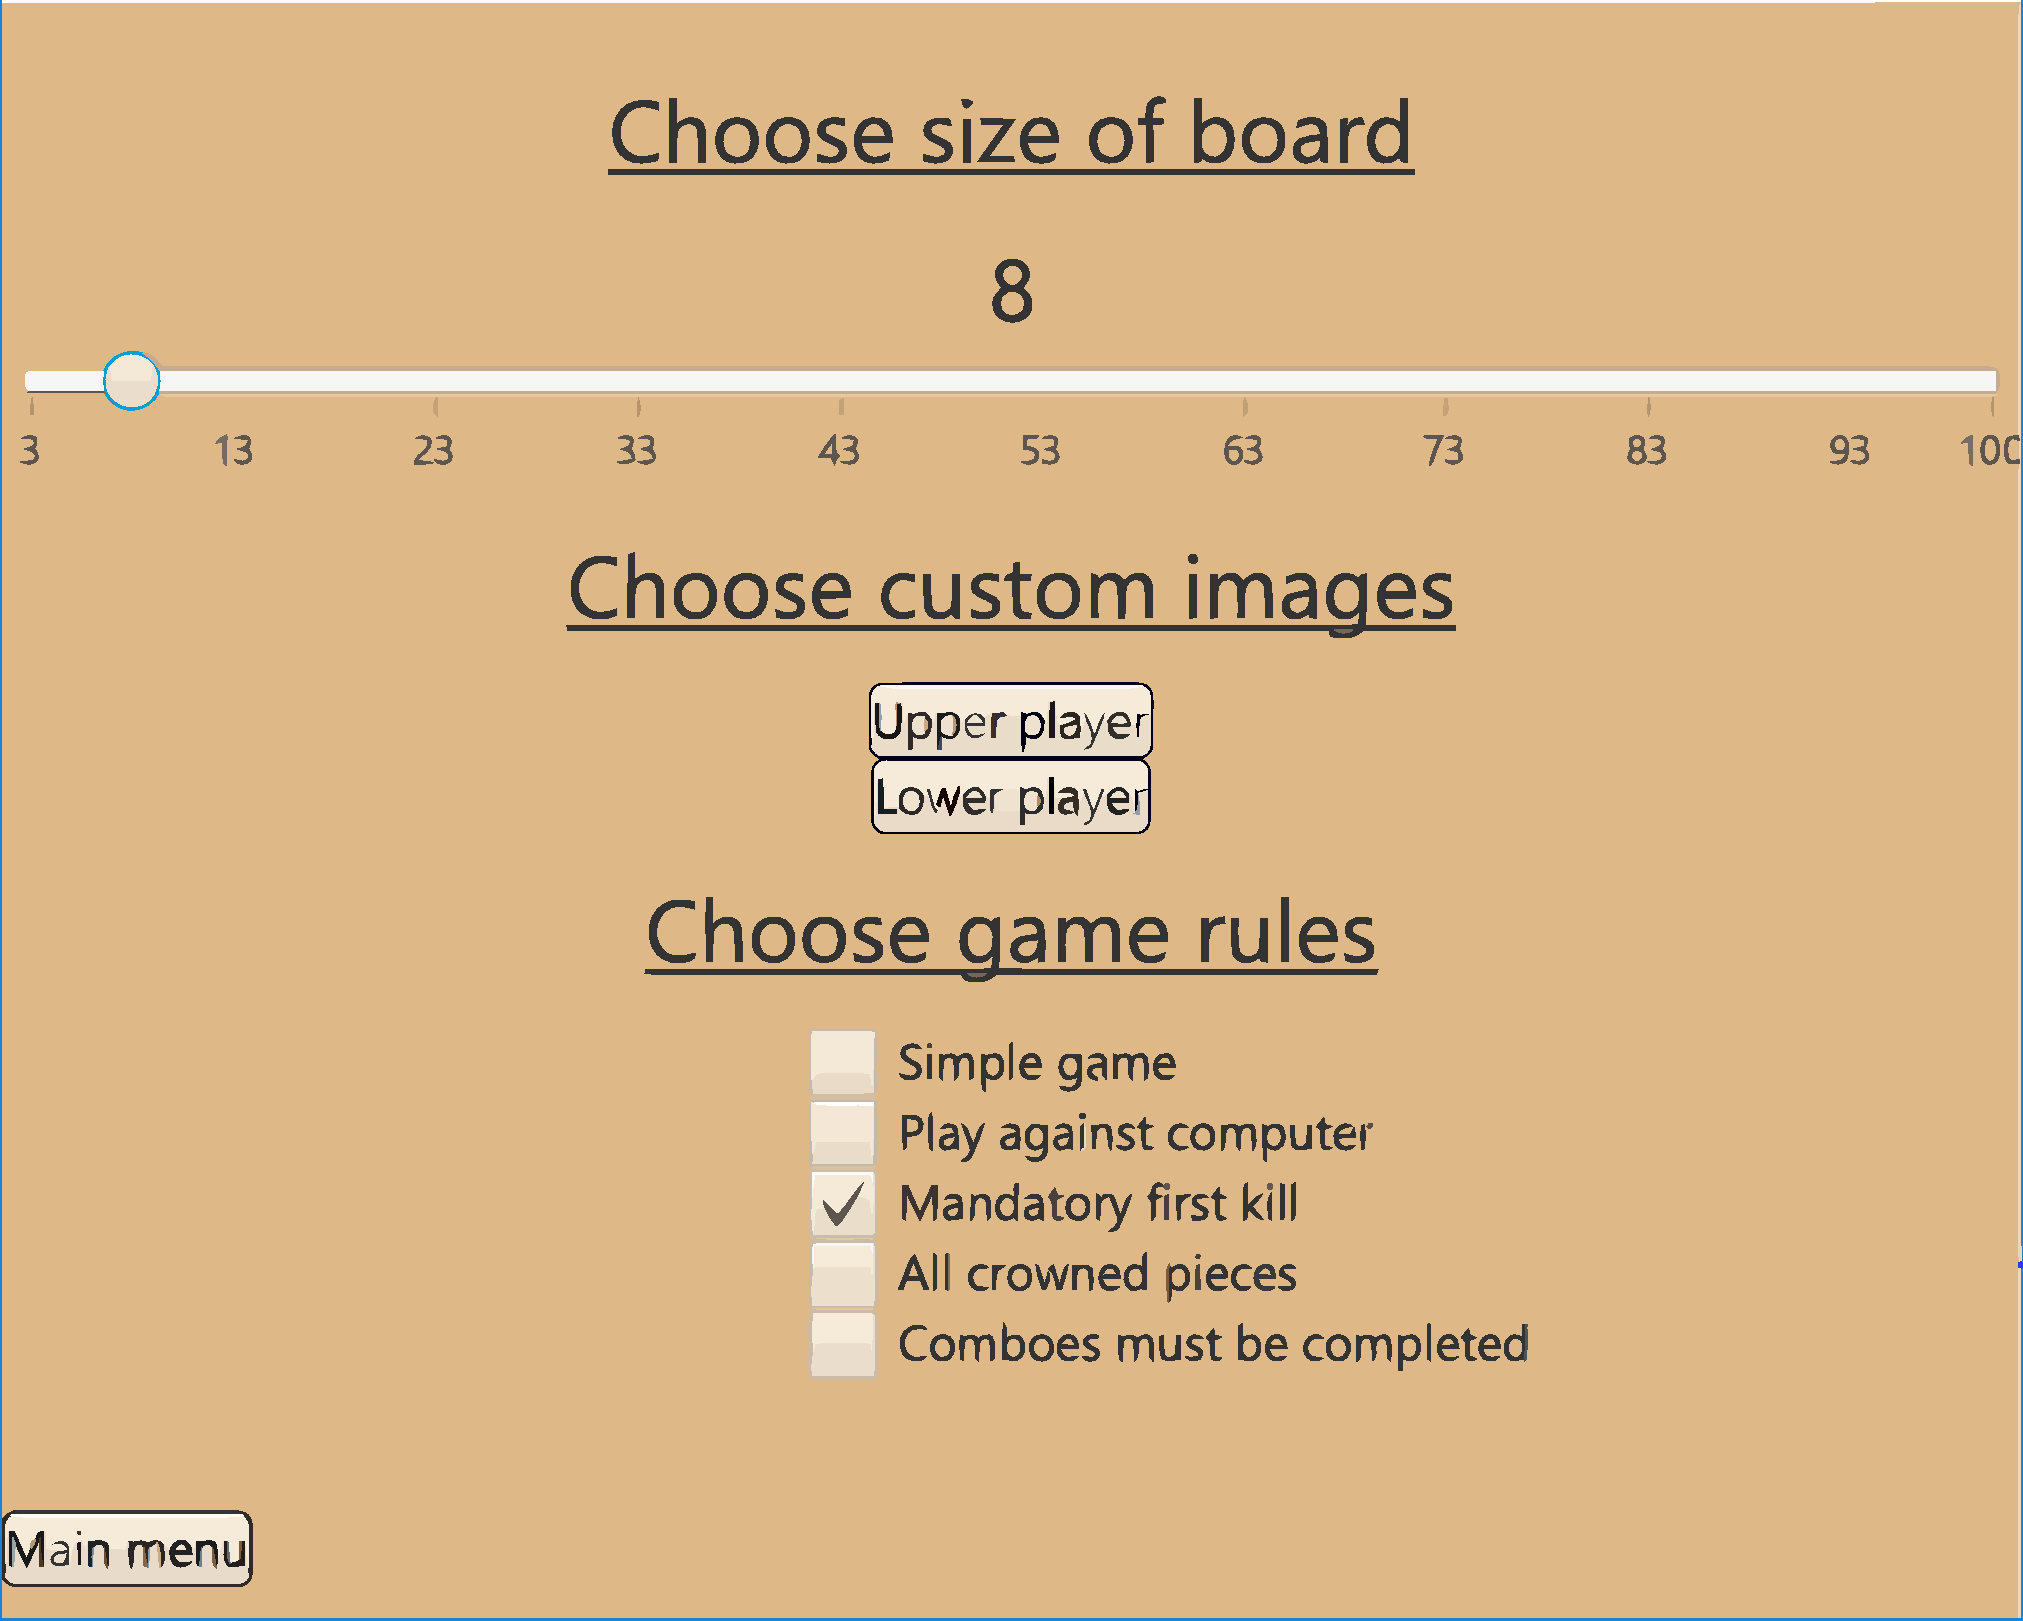
\includegraphics[width = 0.7\textwidth]{Figurer/settingsMenu.pdf}
\caption{Menuen for indstillinger. Her kan vælges brætstørrelse, brikbilleder og diverse spilindstillinger.}
\label{fig:settingsMenu}
\end{figure}